\documentclass[10pt,a4paper]{article}
\usepackage[latin1]{inputenc}
\usepackage{amsmath}
\usepackage{amsfonts}
\usepackage{amssymb}
\usepackage{graphicx}
\author{Morten Sand Knudsen}
\begin{document}
	\section{Android Applikation - JB \& MK}
	I dette afsnit beskrives design og implementring af Traffic Controls android applikation. 
	Applikationen er skrevet i C\# ved hjaelp af Xamarin, som goer dette muligt.
	Til udvikling af vores android applikation er der blevet brugt et MVP design p� en 3-layer arkitektur. Dette kan ses i diagrammet herunder.
	
	\begin{figure} [!ht]
		\begin{center}
			\includegraphics[height=16cm]{MVP}
		\end{center}
		\caption{MVP + 3-layer p� android applikationen}
		\label{fig:MVP}
	\end{figure}
	\pagebreak
	\noindent Model-View-Presenter er et design pattern til opbygning af user interfaces. \textbf{\emph{Model}} er der alt vores data ligger. Det er s� \textbf{\emph{Presenterens}} opgave at manipulere det til \textbf{\emph{Viewet}}. Viewet er det som vi ser som bruger og som vi kan interagere med. Hvis brugeren interagerer med applikationen er det Presenterens opgave at f� det ned i vores Model og f� kaldet det nye view frem. \\
	En �rsag til der er implementeret en MVP p� applikationen er for at g�re koden s� testbar som muligt. \\
	Der er i vores MVP brugt et Observer Pattern som g�r det muligt for vores system at snakke begge veje. Dette er vigtigt da at n�r der kommer opdateringer fra API'et kommer disse med det samme uden at man skal til at lave en refresh p� systemet.
	\\
	\\
	Vi har brugt et 3-layer architetrure pattern til opbygningen af vores applikation. Layers architetruren giver os en logisk opdeling af vores applikation som kan ses p� diagrammet Figure \ref{fig:MVP}.
	\\
	\\
	Der vil p� de kommende sider blive beskrevet hvordan vi har valgt at designe og implementere vores android applikation. Der vil v�re et design, grafisk bruger interface, implenterings og test afsnit til alle delene af vores applikation.
	\pagebreak
	
	\subsection{Navigation i Android applikationen}
	Her er et billede over hvordan man kan navigere rundt i android applikationen. �nskes der et bedre billede af de forskellige activities i android applikationen, kan disse findes i n�ste afsnit Design, implementering og test.
	\begin{figure} [!ht]
		\begin{center}
			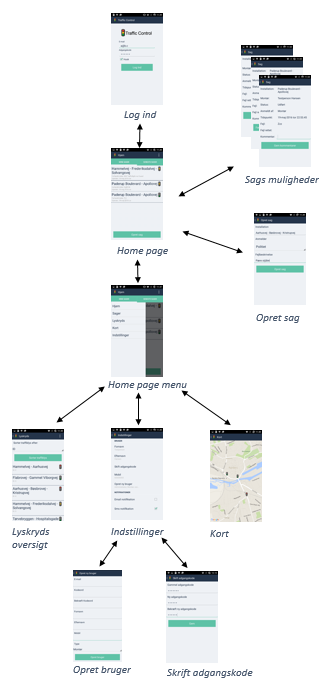
\includegraphics[scale=1.4]{Navigation}
		\end{center}
		\caption{Sekvens diagram for log ind p� android applikationen}
		\label{fig:Navigation i applikationen}
	\end{figure}
	\pagebreak
	
	\subsection{Design, Implementering og Test af Android applikation}
	\subsubsection{Log ind}
	Dette afsnit vil indeholde en gennem gang af design, grafisk bruger interface, implentering og test af Log ind activityen til android applikationen
	\paragraph{Design}
	I dette afsnit ses et sekvens diagram over log ind forl�bet til android applikationen
	\begin{figure} [!ht]
		\begin{center}
			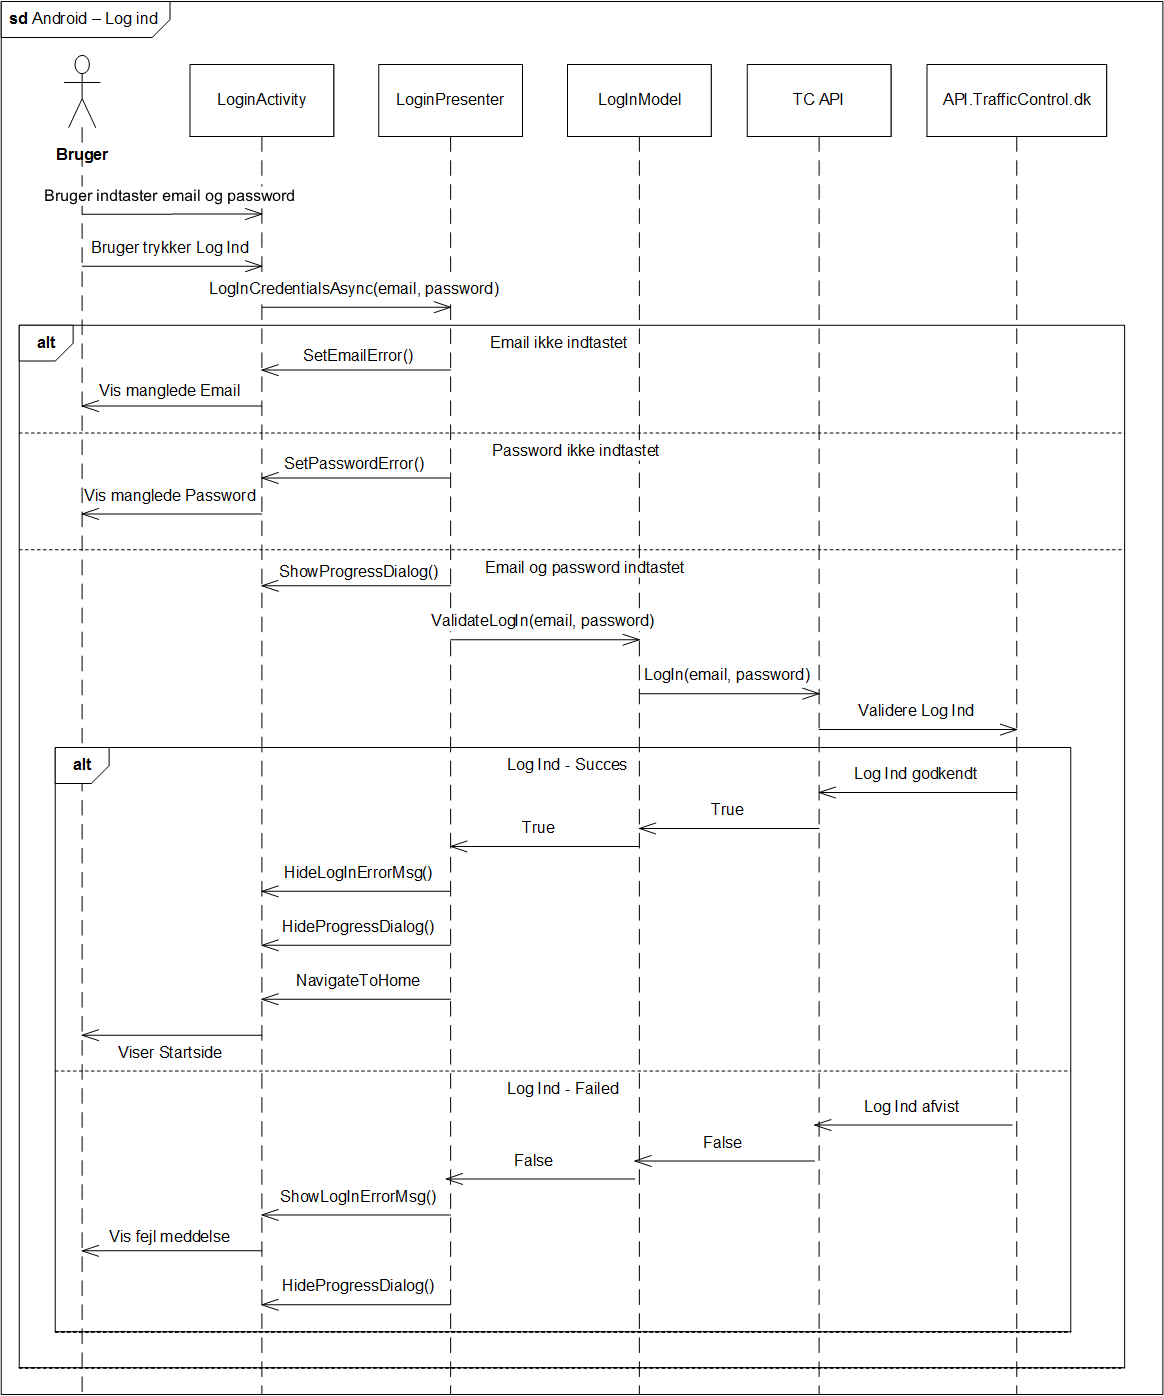
\includegraphics[height=15cm]{SekvensDiagramLogInd}
		\end{center}
		\caption{Sekvens diagram for log ind p� android applikationen}
		\label{fig:Sekvens diagram for Log Ind Android}
	\end{figure}
	\pagebreak
	
	\subsubsection{Grafisk Bruger Interface}
	Her ses hvordan at Log Ind siden ser ud p� android applikationen.
	Det er et meget simpelt design, for at g�re det yderst bruger venligt.
	
	\begin{figure} [h]
		\begin{center}
			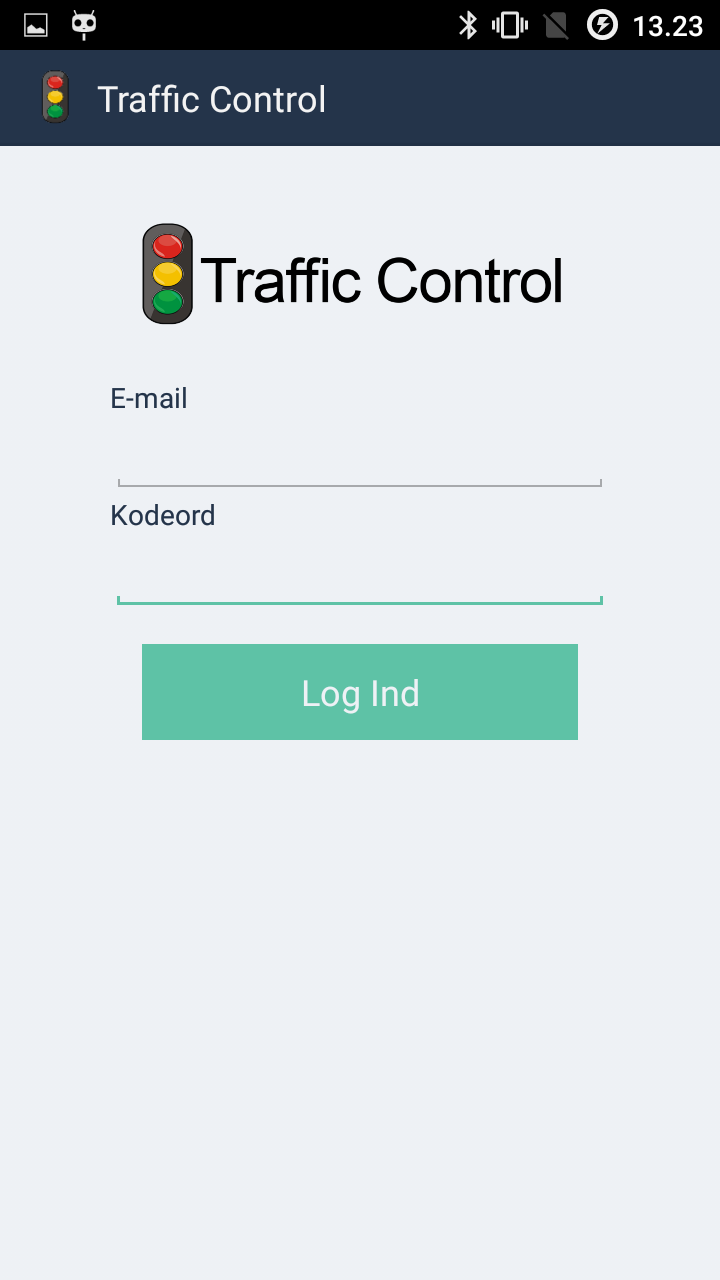
\includegraphics[height=7cm]{AndroidLogIn}
		\end{center}
		\caption{Traffic Control - Log ind}
		\label{fig:Traffic Control - Log ind}
	\end{figure}
	
	\subsubsection{Implementering}
	
	\subsubsection{Test}
	
	Ja tak\\
	
	\pagebreak
	\subsection{Home page}
	Dette afsnit vil indeholde en gennem gang af design, grafisk bruger interface, implentering og test af Home page activityen til android applikationen
	\subsubsection{Design}
	\subsubsection{Grafisk Bruger Interface}
	Hjemsiden er noget mere kompleks end nogle af de andre siger. Dette er fors�gt at gjort simpelt ved ikke at have for mange egenskaber af gangen.
	\begin{figure}[h!]
		\begin{center}
			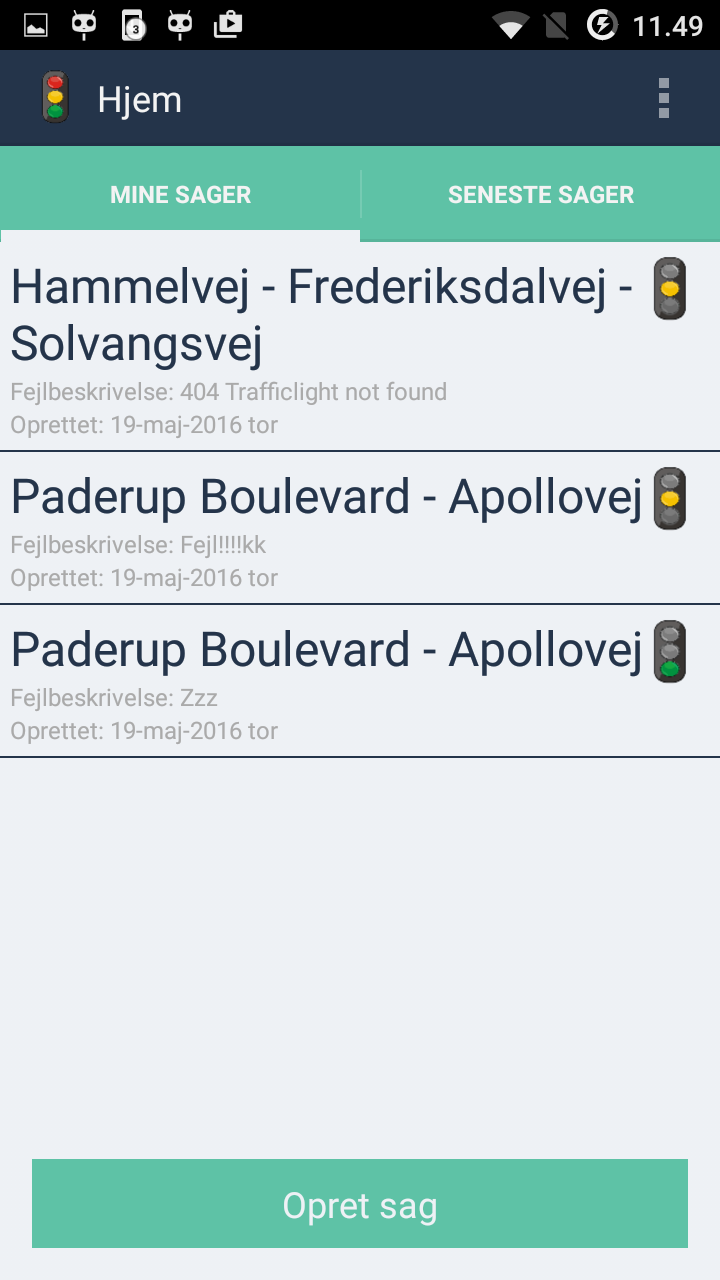
\includegraphics[height=8cm]{AndroidHomePage}
		\end{center}
		\caption{Traffic Control - Home Page}
		\label{fig: Traffic Control - Home Page}
	\end{figure}
	\\
	Hjemsiden indeholder en liste af sager. Trafik lyset ud for sagen viser hvilken status den er i. R�d for lukket, gul for afventer og gr�n for �ben. \\
	Der er to taps hvor man kan v�lge at se alle sager eller om man kun vil se de sager man selv har taget.
	
	\subsubsection{Implementering}
	
	\subsubsection{Test}
	
	Ja tak\\
	\pagebreak
	
	\subsection{Opret bruger}
	Dette afsnit vil indeholde en gennem gang af design, grafisk bruger interface, implentering og test af Opret bruger activityen til android applikationen
	\subsubsection{Design}
	Dette afsnit viser et sekvens diagram over Opret bruger forl�bet i android applikationen
	\begin{figure} [!ht]
		\begin{center}
			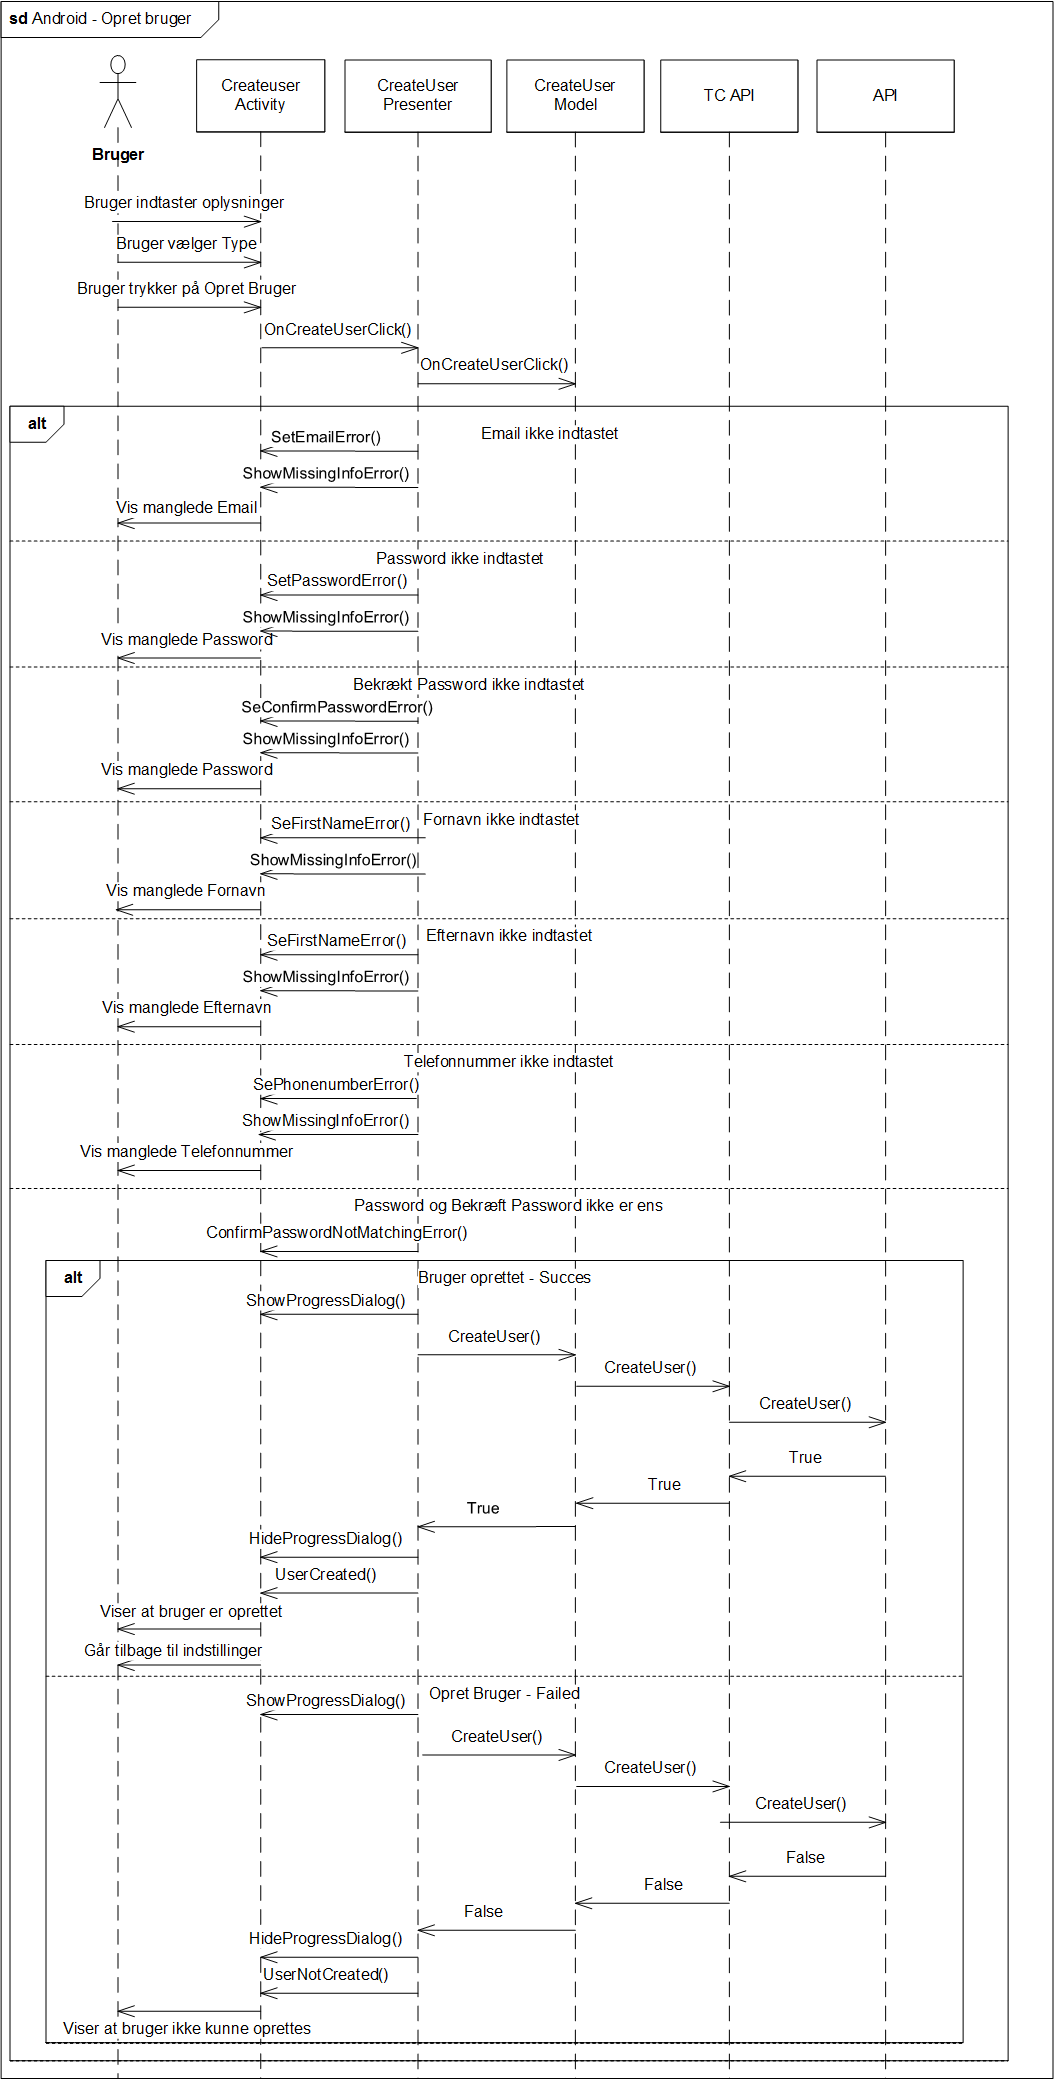
\includegraphics[height=15cm, width=11cm]{OpretBrugerSekvens}
		\end{center}
		\caption{Sekvens diagram for opret bruger p� android applikationen}
		\label{fig:OpretBrugerSekvens}
	\end{figure}
	\pagebreak
	
	\subsubsection{Grafisk Bruger Interface}
	
	\begin{figure}[!ht]
		\begin{center}
			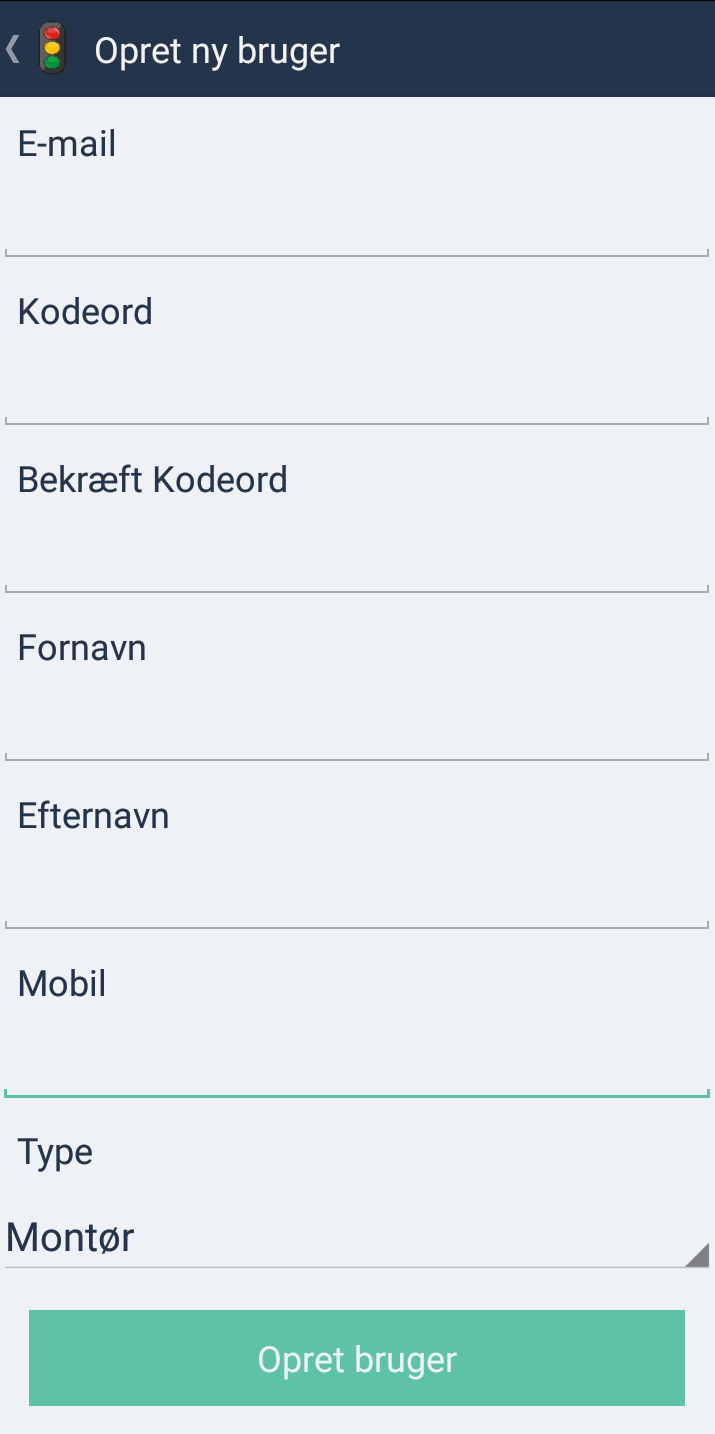
\includegraphics[height=9cm]{AndroidOpretbruger}
		\end{center}
		\caption{Traffic Control - Opret Bruger}
		\label{fig: Traffic Control - Opret Bruger}
	\end{figure}
	
	\noindent Opret bruger siden er igen gjort simpel og nem at arbejde med. Her er lavet felter til alt det info som skal tastes ind om en bruger og til sidst er der lavet en drop down hvor du kan v�lge hvilken type bruger det er.	
	\subsubsection{Implementering}
	
	\subsubsection{Test}
	Ja tak
	\pagebreak
	
\subsection{Lyskryds oversigt}
Dette afsnit vil indeholde en gennem gang af design, grafisk bruger interface og implentering af Lyskryds oversigt activityen til android applikationen
\subsubsection{Design}
I dette afsnit ses et design Lyskryds oversigten til android applikationen
\begin{figure} [!ht]
	\begin{center}
		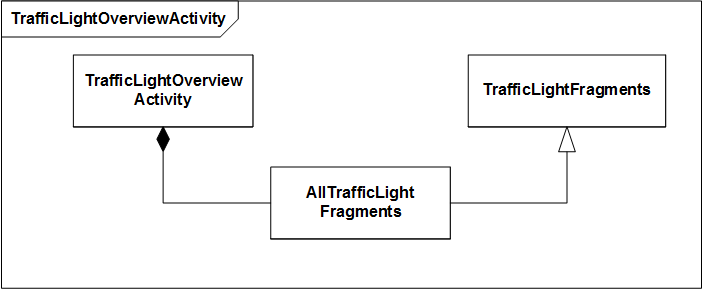
\includegraphics[height=7cm]{Android/Billeder/Lyskryds}
	\end{center}
	\caption{Design over lyskryds oversigten p� android applikationen}
	\label{fig:Design over lyskryds oversigten p� android applikationen}
\end{figure}\\
TrafficLightOverviewActivity er bygget op om samme design som HomeActivity, se figur \vref{fig: Traffic Control - Home Page}. Forskellen mellem Home- og TrafficLightOverviewActivity ligger i at de tabs HomeActivity havde er fjernet. Men derimod har TrafficLightOverviewActivity f�et tilf�jet et felt hvor du kan v�lge en v�rdi du �nsker at sortere lyskrydsene efter.

\pagebreak

\subsubsection{Grafisk Bruger Interface}	
\begin{figure} [!ht]
	\begin{center}
		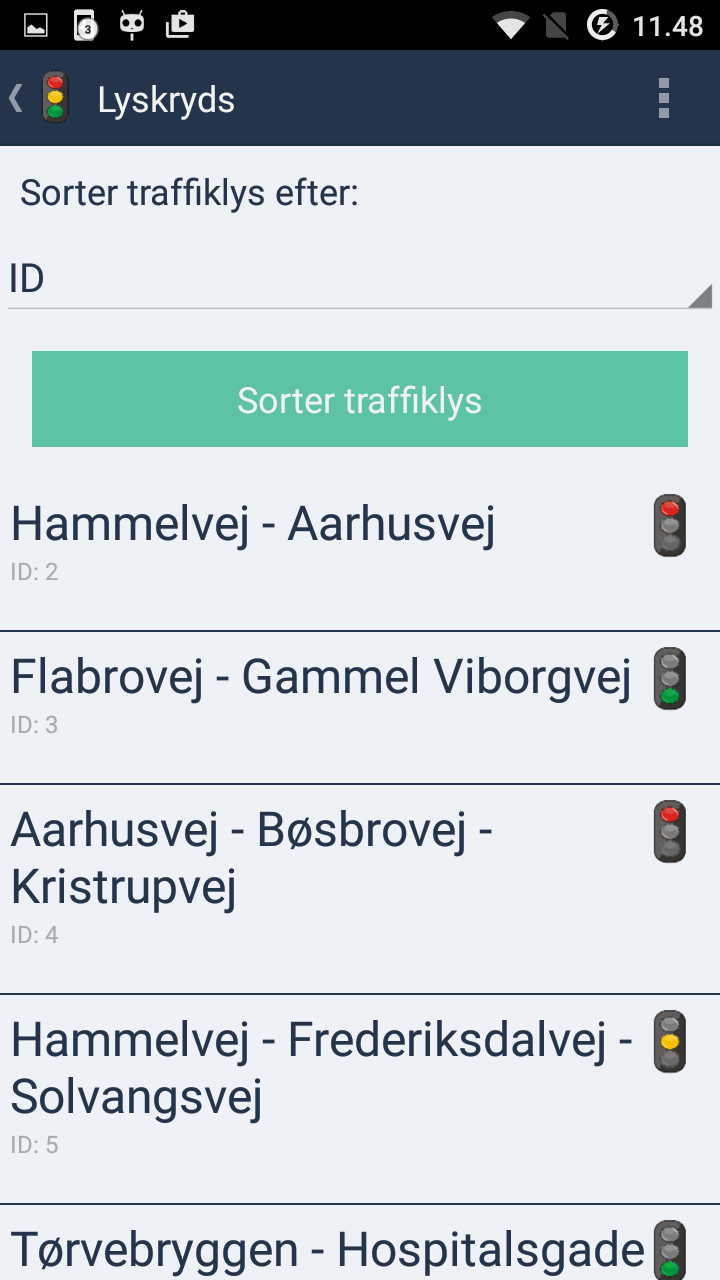
\includegraphics[height=10cm]{Android/Billeder/AndroidLyskryds}
	\end{center}
	\caption{Oversigt over lyskryds p� android applikationen}
	\label{fig:Oversigt over lyskryds p� android applikationen}
\end{figure}

\noindent Denne activity i applikationen bruges til at f� et overblik over alle lyskryds som der er i databasen. Man kan sortere alle lyskryds efter; adresse, ID eller status. Man kan se om der er en sag p� et lyskryds ud fra ikonet ud for en sag, der viser r�d eller gul hvis der er en sag der skal have opm�rksomhed, eller gr�n hvis lyskrydset ingen sager har.\\
Her fra vil man kunne navigere videre til de enkelte lyskryds, hvorfra man kan se lyskryds' status, placering, log og bilag.

\subsubsection{Implementering}
TrafficLightOverviewActivity er bygget op omkring MVP. Modellen indeholder alle de lyskryds der er i Rander Kommune, disse hentes fra DAL-laget.
Der er �verst i TrafficLightOverviewActivity lavet en spinner samt en knap som g�r det muligt at v�lge en v�rdi som �nskes lyskryds sorteret efter.
Under sorterings delen af activityen best�r af to fragments som i Homeactivityen, se \vref{HomePageImp}.


\pagebreak
	\pagebreak
\end{document}